\documentclass[xcolor=dvipsnames,presentation]{beamer}    % ,handout
% colortbl only defines \rowcolor for a single row. xcolor extends this to multiple rows.

\usetheme[sectionoutline]{Aachen} %
\usepackage[ngerman]{babel}
\usepackage[T1]{fontenc}
\usepackage[utf8]{inputenc}

%%%%%%%%%%%%%%%%%%%%%%%%%%%%%%%%%%%%%%%%%%%%%%%%%%%%%%%%%%%%%%%%%%%%%%
% tables
\usepackage{multirow,array,tabularx,rotating}
\usepackage{booktabs}

% math
\usepackage{amsmath,amsthm, amssymb, latexsym, xspace}
\usepackage{bbold}
%\usefonttheme[onlymath]{serif}
%\boldmath

% misc
\usepackage{subfigure}
\usepackage{wasysym}
\usepackage{nameref}

\usepackage{tikz}
\usetikzlibrary{trees,calc}
\usepackage[absolute,overlay]{textpos}

\tikzset{
grow=down,
level 1/.style={sibling distance=7cm, level distance=3cm},
level 2/.style={sibling distance=7cm, level distance=3cm},
level 3/.style={sibling distance=7cm, level distance=3cm},
level 4/.style={sibling distance=7cm, level distance=3cm},
virtual/.style={ultra thick,rectangle,draw=black},
leaf/.style={ultra thick,circle,draw=black},
edge from parent/.style={ultra thick,draw=black},
edge from parent path={
(\tikzparentnode) |-
($(\tikzparentnode)!0.5!(\tikzchildnode)$) -|
(\tikzchildnode)},
}

\tikzstyle{end} = [circle, minimum width=15pt, fill, inner sep=0pt]

\renewcommand*\ttdefault{txtt}


% declare the path(s) where your graphic files are
\graphicspath{./bilder/}
% and their extensions so you won't have to specify these with
% every instance of \includegraphics
\DeclareGraphicsExtensions{.pdf,.jpeg,.png}

% helpers
\newcommand{\argmin}{\operatornamewithlimits{argmin}}
\newcommand{\argmax}{\operatornamewithlimits{argmax}}

%%%%%%%%%%%%%%%%%%%%%%%%%%%%%%%%%%%%%%%%%%%%%%%%%%%%%%%%%%%%%%%%%%%%%%
%%%%%%%%%%%%%%%%%%%%%%%%%%%%%%%%%%%%%%%%%%%%%%%%%%%%%%%%%%%%%%%%%%%%%%

\renewcommand*{\email}{\url{thomas.gatzweiler@rwth-aachen.de}}
% all email address(es) of the authors (used for \TitlePage)

\title[Huffman-Kodierung]{Adaptive Huffman-Kodierung und Anwendungen}

\setbeamertemplate{navigation symbols}{} %disable navigation bar

%% author and in []: shortauthor
\author[Gatzweiler]{Thomas Gatzweiler}
% - Use the \inst{?} command only if the authors have different
%   affiliation.
\institute[RWTH Aachen University] % (optional, but mostly needed)
{
%  \inst{1}%
  \strut Human Language Technology and Pattern Recognition\\
  \strut Computer Science Department, RWTH Aachen University %\\
  %\strut {\tt lehnen@cs.rwth-aachen.de}
}
% - Use the \inst command only if there are several affiliations.
% - Keep it simple, no one is interested in your street address.

\date[12. November 2014]{Proseminar Datenkompression, 12. November 2014, Aachen}

%%%%%%%%%%%%%%%%%%%%%%%%%%%%%%%%%%%%%%%%%%%%%%%%%%%%%%%%%%%%%%%%%%%%%%
% will be set into the PDF document summary
\hypersetup{
  pdftitle={\inserttitle},
  pdfauthor={\insertauthor},
  bookmarksdepth=subsubsection,
  % enable automatic page transitions: for endless loop edit in
  % acrobat reader -> preferences -> full screen -> after every X
  % seconds and after last page
  %pdfpageduration = 2,
  % pdfpagetransition = {Glitter /Di 315 /D 5}
  % pdfpagetransition = {Box /M /O /D 1},
}

%%%%%%%%%%%%%%%%%%%%%%%%%%%%%%%%%%%%%%%%%%%%%%%%%%%%%%%%%%%%%%%%%%%%%%
\usepackage{pdfpcnotes}

%%%%%%%%%%%%%%%%%%%%%%%%%%%%%%%%%%%%%%%%%%%%%%%%%%%%%%%%%%%%%%%%%%%%%%
%%%%%%%%%%%%%%%%%%%%%%%%%%%%%%%%%%%%%%%%%%%%%%%%%%%%%%%%%%%%%%%%%%%%%%

\newenvironment{witemize}{\itemize\setlength{\itemsep}{1em}}{\enditemize}

%%%%%%%%%%%%%%%%%%%%%%%%%%%%%%%%%%%%%%%%%%%%%%%%%%%%%%%%%%%%%%%%%%%%%%
%%%%%%%%%%%%%%%%%%%%%%%%%%%%%%%%%%%%%%%%%%%%%%%%%%%%%%%%%%%%%%%%%%%%%%
\begin{document}
% Literaturverzeichnis wie in der .bib Datei ordnen
\nocite{*}

%%%%%%%%%%%%%%%%%%%%%%%%%%%%%%%%%%%%%%%%%%%%%%%%%%%%%%%%%%%%%%%%%%%%%%
\begin{frame}[label=titlepage]
  \titlepage
\end{frame}

%%%%%%%%%%%%%%%%%%%%%%%%%%%%%%%%%%%%%%%%%%%%%%%%%%%%%%%%%%%%%%%%%%%%%%

% use this, if you use option nosectionoutline
%

\begin{frame}<*>{\iflanguage{ngerman}{Gliederung}{Outline}}
  \tableofcontents[subsectionstyle=show/hide/hide]
\end{frame}

%%%%%%%%%%%%%%%%%%%%%%%%%%%%%%%%%%%%%%%%%%%%%%%%%%%%%%%%%%%%%%%%%%%%%%

%\section{Einführung} \label{sec:intro}
%\begin{frame}{\insertsection}
%Hello World
%\pnote{bla bla bla}
%\end{frame}

%%%%%%%%%%%%%%%%%%%%%%%%%%%%%%%%%%%%%%%%%%%%%%%%%%%%%%%%%%%%%%%%%%%%%%

\begin{frame}[fragile]{Literatur}

  \begin{thebibliography}{}

\bibitem[\protect{Salomon} 10]{Salomon:2010}
D.~Salomon:
\newblock {\em Handbook of Data Compression}.
\newblock Springer, 5th edition, 2010.

\bibitem[\protect{Sayood} 06]{Sayood:2006}
K.~Sayood:
\newblock {\em Introduction to Data Compression}.
\newblock Elsevier, 3rd edition, 2006.

\bibitem[\protect{Bookstein \& Klein} 93]{Bookstein:1993}
A.~Bookstein, S.~Klein: \newblock Is Huffman Coding Dead?
\newblock {\em Computing}, Vol.~50, pp.~279--296, 1993.

\bibitem[\protect{Wallace} 91]{Wallace:1991}
G. K. Wallace: \newblock The {JPEG} still picture compression standard.
\newblock {\em Communications of the ACM}, Vol.~34, pp.~30--44, April 1991.

\bibitem[\protect{Beutelspacher} 05]{Beutelspacher:2005}
A.~Beutelspacher: \newblock Kryptologie, 2005.
\newblock Springer, 7. Auflage, 2005.
\end{thebibliography}

 %\bibliographystyle{alpha}
 %\bibliographystyle{i6bibliostyle}
 %\bibliography{references}
\end{frame}

%%%%%%%%%%%%%%%%%%%%%%%%%%%%%%%%%%%%%%%%%%%%%%%%%%%%%%%%%%%%%%%%%%%%%%

\section{Huffman-Kodierung}

\begin{frame}{\insertsection}
  \begin{textblock}{8}(9,4.5)
    \begin{figure}
      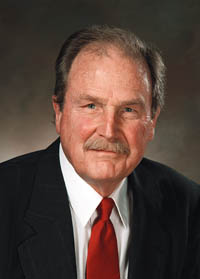
\includegraphics[width=6cm]{bilder/huffman.jpg}
    \end{figure}
    \vspace{-1em}
    \begin{center}
      David Huffman
    \end{center}
  \end{textblock}

  \pnote{Grundlage für die adaptive Huffman-Kodierung}
  \begin{witemize}
    \item 1952 von David Huffman entwickelt
    \pnote{Huffman: amerikanischer Informatiker 1925-1999}
    \item Entropiekodierung
      \begin{itemize}
        \item Seltene Symbole $\Rightarrow$ Lange Codewörter
        \item Häufige Symbole $\Rightarrow$ Kurze Codewörter
      \end{itemize}
    \item Verlustfreie Komprimierung
    \item Erzeugt präfixfreien Code
      \pnote{David Huffman: 1925-1999}
      \pnote{Entropiekodierung: stochastische Kodierung}
      \pnote{Symbole aus einem Eingabealphabet werden Codewörter zugewiesen}
      \pnote{Kein Codewort ist Präfix eines anderen Codeworts}
      \pnote{Vorteil: Codewörter lassen sich direkt hintereinander schreiben}
  \end{witemize}
\end{frame}

\subsection{Huffman-Baum}

\begin{frame}{\insertsubsection}
  \begin{witemize}
  \item Zentrale Datenstruktur
  \item Binärbaum $\Rightarrow$ binärer Codes
    \pnote{Lässt sich auch auf andere Zahlensysteme anwenden}
  \item Basiert auf Wahrscheinlichkeitsverteilung des Eingabealphabets
    \pnote{Wahrscheinlichkeiten können geschätzt oder vorher ermittelt
      werden (diskret)}
  \item Aufbau von unten nach oben
    \pnote{Kodierung ist präfixfrei, da die Symbole nur in den Blättern stehen}
  \end{witemize}
\end{frame}

\begin{frame}{\insertsubsection: Konstruktion}
  \begin{witemize}
  \item Sortierung der Liste des Eingabealphabets nach Wahrscheinlichkeiten
  \item Die zwei seltensten Symbole werden aus der Liste entfernt
  \item Erzeugung je eines Blattknotens für die zwei Symbole
  \item Erzeugung eines Elternknotens für die zwei Blattknoten
  \item Einfügen eines Hilfssymbols mit der summiertern
    Wahrscheinlichkeit beider Symbole in die Liste
  \item Wiederholung bis ein Hilfssymbol übrig bleibt
  \end{witemize}
\end{frame}

\begin{frame}[fragile]{\insertsubsection: Beispiel}

\begin{textblock}{5}(10,3)
\begin{flushright}
\begin{tabular}{l|l}
$a_i$ & $P(a_i)$ \\ \hline
\only<1>
{A & 0.20 \\
B & 0.06 \\
C & 0.10 \\
D & 0.14 \\
E & 0.50}\only<2>
{E & 0.50 \\
A & 0.20 \\
D & 0.14 \\
C & 0.10 \\
B & 0.06}\only<3-4>
{E & 0.50 \\
A & 0.20 \\
D & 0.14 \\
\color{red}C & \color{red}0.10 \\
\color{red}B & \color{red}0.06}\only<5>
{E & 0.50 \\
A & 0.20 \\
\color{ForestGreen}\{C, B\} & \color{ForestGreen}0.16 \\
D & 0.14}\only<6-7>
{E & 0.50 \\
A & 0.20 \\
\color{red}\{C, B\} & \color{red}0.16 \\
\color{red}D & \color{red}0.14}\only<8>
{E & 0.50 \\
\color{ForestGreen}\{B, C, D\} & \color{ForestGreen}0.30 \\
A & 0.20}\only<9-10>
{E & 0.50 \\
\color{red}\{B, C, D\} & \color{red}0.30 \\
\color{red}A & \color{red}0.20}\only<11>
{E & 0.50 \\
\color{ForestGreen}\{A, B, C, D\} & \color{ForestGreen}0.50}\only<12-13>
{\color{red}E & \color{red}0.50 \\
\color{red}\{A, B, C, D\} & \color{red}0.50}\only<14-15>
{\color{ForestGreen}\{A, B, C, D, E\} & \color{ForestGreen}1.00}
\end{tabular}
\end{flushright}
\end{textblock}

\begin{tikzpicture}[
level 1/.style={sibling distance=8cm, level distance=3.5cm},
level 2/.style={sibling distance=6cm, level distance=3.5cm},
level 3/.style={sibling distance=6cm, level distance=3.5cm},
level 4/.style={sibling distance=6cm, level distance=3.5cm},
]
\tikzstyle{lvl8}=[transparent]
\tikzstyle{lvl7}=[transparent]
\tikzstyle{lvl6}=[transparent]
\tikzstyle{lvl5}=[transparent]
\tikzstyle{lvl4}=[transparent]
\tikzstyle{lvl3}=[transparent]
\tikzstyle{lvl2}=[transparent]
\tikzstyle{lvl1}=[transparent]
\tikzstyle{lvl0}=[transparent]
\only<4->{\tikzstyle{lvl0}=[opaque]}
\only<5->{\tikzstyle{lvl1}=[opaque]}
\only<7->{\tikzstyle{lvl2}=[opaque]}
\only<8->{\tikzstyle{lvl3}=[opaque]}
\only<10->{\tikzstyle{lvl4}=[opaque]}
\only<11->{\tikzstyle{lvl5}=[opaque]}
\only<13->{\tikzstyle{lvl6}=[opaque]}
\only<14->{\tikzstyle{lvl7}=[opaque]}
\only<15->{\tikzstyle{lvl8}=[opaque]}
\node[virtual,lvl7] {\{A, B, C, D, E\}}
child[lvl6] {
  node[leaf] {E}
  edge from parent
  node[left,lvl8] {\small$0.50$}
}
child[lvl6] {
  node[virtual,lvl5] {\{A, B, C, D\}}
  child[lvl4] {
    node[virtual,lvl3] {\{B, C, D\}}
    child[lvl2] {
      node[virtual,lvl1] {\{C, B\}}
      child[lvl0] {
        node[leaf] {C}
        edge from parent
        node[left,lvl8] {\small$0.10$}
      }
      child[lvl0] {
        node[leaf] {B}
        edge from parent
        node[right,lvl8] {\small$0.06$}
      }
      edge from parent
      node[left,lvl8] {\small$0.16$}
    }
    child[lvl2] {
      node[leaf] {D}
      edge from parent
      node[right,lvl8] {\small$0.14$}
    }
    edge from parent
    node[left,lvl8] {\small$0.30$}
  }
  child[lvl4] {
    node[leaf] {A}
    edge from parent
    node[right,lvl8] {\small$0.20$}
  }
  edge from parent
  node[right,lvl8] {\small$0.50$}
};
\end{tikzpicture}
\end{frame}


\subsection{Kodierung}

\begin{frame}{\insertsubsection}
  \begin{witemize}
  \item Codewort: Pfad von der Wurzel zum Blatt
  \item Linker Teilbaum: {\tt1} wird angehängt
  \item Rechter Teilbaum: {\tt0} wird angehängt
  \item Oder umgekehrt (implementationsabhängig)
  \end{witemize}
\end{frame}

\begin{frame}{\insertsubsection: Beispiel}
\begin{textblock}{5}(10,3)
\begin{flushright}
\begin{tabular}{l|l}
$a_i$ & $C(a_i)$ \\ \hline
\only<2->
{\only<2>{\color{i6blue}}A & \only<2>{\color{i6blue}}{\tt00} \\}
\only<3->
{\only<3>{\color{i6blue}}B & \only<3>{\color{i6blue}}{\tt0110} \\}
\only<4->
{\only<4>{\color{i6blue}}C & \only<4>{\color{i6blue}}{\tt0111} \\}
\only<5->
{\only<5>{\color{i6blue}}D & \only<5>{\color{i6blue}}{\tt010} \\}
\only<6->
{\only<6>{\color{i6blue}}E & \only<6>{\color{i6blue}}{\tt1} \\}
\end{tabular}
\end{flushright}
\end{textblock}

\only<8-9>{
\begin{textblock}{8}(9,12)
$C(EBBE) = \only<9>{\tt1011001101}$
\end{textblock}
}

\begin{tikzpicture}[
level 1/.style={sibling distance=8cm, level distance=3.5cm},
level 2/.style={sibling distance=6cm, level distance=3.5cm},
level 3/.style={sibling distance=6cm, level distance=3.5cm},
level 4/.style={sibling distance=6cm, level distance=3.5cm},
]
\tikzstyle{A}=[]
\tikzstyle{B}=[]
\tikzstyle{C}=[]
\tikzstyle{D}=[]
\tikzstyle{E}=[]
\only<2>{\tikzstyle{A}=[i6blue,line width=8pt]}
\only<3>{\tikzstyle{B}=[i6blue,line width=8pt]}
\only<4>{\tikzstyle{C}=[i6blue,line width=8pt]}
\only<5>{\tikzstyle{D}=[i6blue,line width=8pt]}
\only<6>{\tikzstyle{E}=[i6blue,line width=8pt]}
\node[virtual] {\{A, B, C, D, E\}}
child {
  node[leaf] {E}
  edge from parent[E]
  node[left] {\tt1}
}
child {
  node[virtual] {\{A, B, C, D\}}
  child {
    node[virtual] {\{B, C, D\}}
    child {
      node[virtual] {\{C, B\}}
      child {
        node[leaf] {C}
        edge from parent[C]
        node[left] {\tt1}
      }
      child {
        node[leaf] {B}
        edge from parent[B]
        node[right] {\tt0}
      }
      edge from parent[B,C]
      node[left] {\tt1}
    }
    child {
      node[leaf] {D}
      edge from parent[D]
      node[right] {\tt0}
    }
    edge from parent[B,C,D]
    node[left] {\tt1}
  }
  child {
    node[leaf] {A}
    edge from parent[A]
    node[right] {\tt0}
  }
  edge from parent[A,B,C,D]
  node[right] {\tt0}
};
\end{tikzpicture}
\end{frame}

\subsection{Dekodierung}

\begin{frame}{\insertsubsection}
  \begin{witemize}
  \item Benötigt Huffman-Baum oder Wahrscheinlichkeitsverteilung
    \pnote{Baum oder Verteilung muss mit den kodierten Daten
      gespeichert oder übertragen werden}
  \item Aufbau des Huffman-Baums wie beim Kodierer
  \item Dekodierer startet bei der Wurzel, ließt die Daten bitweise
    \begin{itemize}
    \item {\tt1} eingelesen: Zum linken Nachfolger gehen
    \item {\tt0} eingelesen: Zum rechten Nachfolger gehen
    \item Oder umgekehrt (wie beim Kodierer)
    \end{itemize}
  \item Blatt erreicht: Symbol ausgeben und zur Wurzel zurückkehren
  \end{witemize}
\end{frame}

\section{Adaptive Huffman-Kodierung}

\begin{frame}{\insertsection}
  \begin{witemize}
  \item Huffman-Kodierung:
    \begin{itemize}
      \item Wahrscheinlichkeitsverteilung muss bekannt sein
      \item Echtzeitkodierung nicht möglich
    \end{itemize}
  \item Lösung: Adaptive Huffman-Kodierung
    \begin{itemize}
    \item 1973 von Newton Faller und 1978 von Robert Gallager
      unabhängig entwickelt
    \item 1985 von Donald Knuth wesentlich verbessert
    \pnote{Basiert auf der Huffman-Kodierung}
    \item Kodierung ohne Verzögerung, in einem Durchgang
    \pnote{Jedes Eingangssymbol erzeugt sofort ein Codewort}
    \item Passt sich laufend der Häufigkeitsverteilung an
    \end{itemize}
  \end{witemize}
\end{frame}

\begin{frame}{\insertsection}
  \begin{witemize}
  \item Start mit leerem Huffman-Baum
  \item Knoten haben Häufigkeitszähler (Integer)
  \item Neue Häufigkeitsverteilung $\Rightarrow$ Aktualisierung des
    Huffman-Baums
  \item Kodierer und Dekodierer spiegeln Operationen auf Huffman-Baum
  \end{witemize}
\end{frame}

\subsection{Kodierung}

\begin{frame}{\insertsubsection}
  \begin{witemize}
  \item Unbekanntes Symbol:
    \begin{itemize}
    \item Unkodiert ausgeben
    \item In den Huffman-Baum einfügen
    \end{itemize}

  \item Bekanntes Symbol:
    \begin{itemize}
    \item Codewort ausgeben
    \item Huffman-Baum aktualisieren
    \end{itemize}
  \end{witemize}
\end{frame}

\subsection{Dekodierung}

\begin{frame}{\insertsubsection}
  \begin{witemize}
  \item Spiegelt die Änderungen des Huffman-Baums vom Kodierer
  \item Unkodiertes Symbol:
    \begin{itemize}
      \item Direkt wieder ausgeben
      \item In den Huffman-Baum einfügen
    \end{itemize}
  \item Kodiertes Symbol:
    \begin{itemize}
    \item Dekodiertes Symbol ausgeben
    \item Huffman-Baum aktualisieren
    \end{itemize}
  \end{witemize}
\end{frame}

\begin{frame}{\insertsection}
  \begin{witemize}
    \item Problem: Unterscheidung von Codewörtern und unkodierten
      Symbolen
    \item Lösung: Benutzung eines speziellen Escape-Codes
    \item Neue Probleme:
      \begin{itemize}
      \item Escape-Code darf kein Codewort und kein Präfix davon sein
      \item Codewörter ändern sich laufend
      \end{itemize}
    \item Lösung: Escape-Code als Symbol im Huffman-Baum verwalten
      \pnote{Codewort des Escape-Codes passt sich automatisch der
        Häufigkeit neuer Symbole an}
  \end{witemize}
\end{frame}

\begin{frame}[<+->]{Escape-Code im Huffman-Baum}
\begin{figure}
\begin{tikzpicture}
\node {}
child {
  node[leaf] {A}
  edge from parent
  node[left]  {\tt1}
}
child {
  child {
    node[leaf] {B}
    edge from parent
    node[left] {\tt1}
  }
  child {
    child {
      node[end] {}
      edge from parent
      node[left] {\tt1}
    }
    child {
      node[leaf] {C}
      edge from parent
      node[right] {\tt0}
    }
    edge from parent
    node[right] {\tt0}
  }
  edge from parent
  node[right] {\tt0}
};
\end{tikzpicture}
\end{figure}
Escape-Code: {\tt001}
\pnote{Vorteile der Verwaltung des Escape-Codes im Huffman-Baum}
\end{frame}

\subsection{Aktualisierung des Huffman-Baums}

\begin{frame}{\insertsubsection}
  \begin{witemize}
  \item Häufigkeiten müssen monoton steigen, \\
    zeilenweise von rechts unten nach links oben
  \item Prüfung des Huffman-Baums bei jeder Änderung
  \item Wenn notwendig Huffman-Baum anpassen
  \end{witemize}
\end{frame}

\begin{frame}{\insertsubsection}
\begin{figure}
\centering
\begin{tikzpicture}
\node {70}[
level 1/.style={sibling distance=8cm, level distance=3.5cm},
level 2/.style={sibling distance=6cm, level distance=3.5cm},
level 3/.style={sibling distance=3cm, level distance=3.5cm},
]
child {
  node[leaf] {A}
  edge from parent
  node[left] {39}
}
child {
  child {
    child {
      node[leaf] {B}
      edge from parent
      node[left] {8}
    }
    child {
      node[leaf] {C}
      edge from parent
      node[right] {8}
    }
    edge from parent
    node[left] {16}
  }
  child {
    child {
      node[leaf] {D}
      edge from parent
      node[left] {8}
    }
    child {
      node[leaf] {E}
      edge from parent
      node[right] {7}
    }
    edge from parent
    node[right] {15}
  }
  edge from parent
  node[right] {31}
};
\end{tikzpicture}
\end{figure}
\end{frame}

\begin{frame}{\insertsubsection: Algorithmus}
  Der Häufigkeitszähler $F$ von Blattknoten $X$ soll inkrementiert werden.

  \vspace{1cm}

  \begin{enumerate}
  \item Existiert von rechts unten nach links oben gesehen ein
    Nachfolger von $X$ mit einem Häufigkeitszähler $\leq F$, tausche
    $X$ mit dem letzten dieser Nachfolger.

    \emph{Ausnahme:} $X$ darf nicht mit dem Elternknoten getauscht werden
  \item Inkrementiere den Häufigkeitszähler des Knotens $X$ von $F$ auf $F+1$

  \item Ist $X$ der Wurzelknoten, stoppe die Ausführung, sonst führe
    den Algorithmus auf dem Elternknoten von $X$ aus.
  \end{enumerate}

  \vspace{1cm}

  Komplexität: $\mathcal{O}(n \cdot log(n))$
\end{frame}

\begin{frame}{\insertsubsection}
\begin{figure}
\centering
\begin{tikzpicture}
\node {70}[
level 1/.style={sibling distance=8cm, level distance=3.5cm},
level 2/.style={sibling distance=6cm, level distance=3.5cm},
level 3/.style={sibling distance=3cm, level distance=3.5cm},
]
child {
  node[leaf] {A}
  edge from parent
  node[left] {39}
}
child {
  child {
    child {
      node[leaf] {B}
      edge from parent
      node[left] {8}
    }
    child {
      node[leaf] {C}
      edge from parent
      node[right] {8}
    }
    edge from parent
    node[left] {16}
  }
  child {
    child {
      node[leaf] {D}
      edge from parent
      node[left] {8}
    }
    child {
      node[leaf] {E}
      edge from parent
      node[right] {7}
    }
    edge from parent
    node[right] {15}
  }
  edge from parent
  node[right] {31}
};
\end{tikzpicture}
\end{figure}
\end{frame}

\begin{frame}{\insertsubsection}
\begin{figure}
\centering
\begin{tikzpicture}
\node {71}[
level 1/.style={sibling distance=8cm, level distance=3.5cm},
level 2/.style={sibling distance=6cm, level distance=3.5cm},
level 3/.style={sibling distance=3cm, level distance=3.5cm},
]
child {
  node[leaf] {A}
  edge from parent
  node[left] {39}
}
child {
  child {
    child {
      node[leaf] {B}
      edge from parent
      node[left] {8}
    }
    child {
      node[leaf] {C}
      edge from parent
      node[right] {8}
    }
    edge from parent
    node[left] {16}
  }
  child {
    child {
      node[leaf] {D}
      edge from parent
      node[left] {8}
    }
    child {
      node[leaf] {E}
      edge from parent
      node[right] {8}
    }
    edge from parent
    node[right] {16}
  }
  edge from parent
  node[right] {32}
};
\end{tikzpicture}
\end{figure}
\end{frame}

\begin{frame}{\insertsubsection}
\begin{figure}
\centering
\begin{tikzpicture}[
level 1/.style={sibling distance=8cm, level distance=3.5cm},
level 2/.style={sibling distance=6cm, level distance=3.5cm},
level 3/.style={sibling distance=3cm, level distance=3.5cm},
]
\node {72}
child {
  node[leaf]{A}
  edge from parent
  node[left] {39}
}
child {
  child {
    child {
      node[leaf](X) {E}
      edge from parent
      node[left] {9}
    }
    child {
      node[leaf] {C}
      edge from parent
      node[right] {8}
    }
    edge from parent
    node[left] {17}
  }
  child {
    child {
      node[leaf] {D}
      edge from parent
      node[left] {8}
    }
    child {
      node[leaf](Y) {B}
      edge from parent
      node[right] {8}
    }
    edge from parent
    node[right] {16}
  }
  edge from parent
  node[right] {33}
};
\draw[<->, dashed, ultra thick] (Y.north west) to[out=130,in=50,looseness=1.5] (X.north east);
\end{tikzpicture}
\end{figure}
\end{frame}

\subsection{Überlauf der Häufigkeitszähler}

\begin{frame}{\insertsubsection}
  \begin{witemize}
  \item Häufigkeitszähler sind Integer
  \item Integerüberlauf bei großen Datenmengen
  \item Lösung: Skalierung der Häufigkeitszähler
    \begin{itemize}
    \item Häufgkeitszähler werden durch 2 geteilt $\Rightarrow$ Right-Shift
    \item Huffmanbaum muss evtl. neu geordnet werden
    \end{itemize}
  \end{witemize}
\end{frame}

\begin{frame}{\insertsubsection}
\begin{figure}
\centering
\begin{tikzpicture}[
level 1/.style={sibling distance=8cm, level distance=3.5cm},
level 2/.style={sibling distance=3cm, level distance=3.5cm},
]
\node {930}
child {
  child {
    node {A}
    edge from parent
    node[left] {310}
  }
  child {
    node {B}
    edge from parent
    node[right] {310}
  }
  edge from parent
  node[left] {620}
}
child {
  child {
    node {C}
    edge from parent
    node[left] {155}
  }
  child {
    node {D}
    edge from parent
    node[right] {155}
  }
  edge from parent
  node[right] {310}
};
\end{tikzpicture}
\end{figure}
\end{frame}

\begin{frame}{\insertsubsection}
\begin{figure}
\centering
\begin{tikzpicture}[
level 1/.style={sibling distance=8cm, level distance=3.5cm},
level 2/.style={sibling distance=3cm, level distance=3.5cm},
]
\node {464}
child {
  child {
    node[leaf] {A}
    edge from parent
    node[left] {155}
  }
  child {
    node[leaf] {B}
    edge from parent
    node[right] {155}
  }
  edge from parent
  node[left] {310}
}
child {
  child {
    node[leaf] {C}
    edge from parent
    node[left] {77}
  }
  child {
    node[leaf] {D}
    edge from parent
    node[right] {77}
  }
  edge from parent
  node[right,red] {\textbf{154}}
};
\end{tikzpicture}
\end{figure}
\end{frame}

\section{Anwendungen}

\begin{frame}{\insertsection}
  \begin{witemize}
  \item Huffman-Kodierung wird meist adaptiv verwendet
  \item Häufig Teil eines mehrstufigen Prozesses
  \item Beispiele:
    \begin{itemize}
    \item Unix-Tool {\tt{compact}}
    \item Letzte Stufe der JPEG-Komprimierung
    \item Teil der MP3- und AAC-Komprimierung
    \end{itemize}
  \end{witemize}
\end{frame}

\subsection{Textkompression}

\begin{frame}{\insertsubsection}
  \begin{witemize}
  \item Einfachster Anwendungsfall
  \item Festes Eingabealphabet (z.B. ASCII)
  \item Erweiterung: Bigramme, Silben oder Wörter als Symbole
  \end{witemize}
\end{frame}

\begin{frame}{\insertsubsection}
  \begin{columns}[T]
    \column{.5\textwidth}
    \begin{tabular}{c|c|l}
      $a_i$ & $P(a_i)$ & $C(a_i)$ \\ \hline
      E & $0.1740$ & {\tt111} \\
      N & $0.0978$ & {\tt001} \\
      I & $0.0755$ & {\tt1101} \\
      S & $0.0727$ & {\tt1011} \\
      R & $0.0700$ & {\tt1010} \\
      A & $0.0651$ & {\tt1001} \\
      T & $0.0615$ & {\tt0111} \\
      D & $0.0508$ & {\tt0101} \\
      H & $0.0476$ & {\tt0001} \\
      U & $0.0435$ & {\tt0000} \\
      L & $0.0344$ & {\tt10001} \\
      C & $0.0306$ & {\tt10000} \\
      G & $0.0301$ & {\tt01101} \\
      M & $0.0253$ & {\tt01001} \\
    \end{tabular}

    \column{.5\textwidth}
    \begin{tabular}{c|c|l}
      $a_i$ & $P(a_i)$ & $C(a_i)$ \\ \hline
      O & $0.0251$ & {\tt01000} \\
      W & $0.0189$ & {\tt110001} \\
      B & $0.0189$ & {\tt110010} \\
      F & $0.0166$ & {\tt110000} \\
      K & $0.0121$ & {\tt011000} \\
      Z & $0.0113$ & {\tt1100111} \\
      P & $0.0079$ & {\tt1100110} \\
      V & $0.0067$ & {\tt0110011} \\
      ß & $0.0031$ & {\tt01100100} \\
      J & $0.0027$ & {\tt011001011} \\
      Y & $0.0004$ & {\tt0110010100} \\
      X & $0.0003$ & {\tt01100101011} \\
      Q & $0.0002$ & {\tt01100101010}
    \end{tabular}
  \end{columns}
  \vspace{15pt}
  \emph{Kompressionsrate: 82.5\%}
\end{frame}

\subsection{Verlustfreie Bildkompression}

\begin{frame}{\insertsubsection}
\begin{witemize}
\item<1-> 1-Bit Schwarzweißbilder
  \begin{itemize}
    \item Keine Komprimierung möglich
    \item {\tt0}: Schwarz, {\tt1}: Weiß
  \end{itemize}

\item<2-> 8-Bit Graustufenbilder
  \begin{itemize}
    \item Einfachster Anwendungsfall
    \item {\tt0}: Schwarz, {\tt1-254}: Graustufen, {\tt255}: Weiß
  \end{itemize}

\item<3-> Farbbilder
  \begin{itemize}
    \item Ein Huffman-Baum pro Farbkanal möglich
    \item Korrelation zwischen Farbkanälen bleibt unberücksichtigt
  \end{itemize}
\end{witemize}
\end{frame}

\begin{frame}{\insertsubsection}
\begin{figure}[T]
  \centering
  
\includegraphics[width=0.470\textwidth]{bilder/uniformnoise.png}
  \hfill
  \only<2>{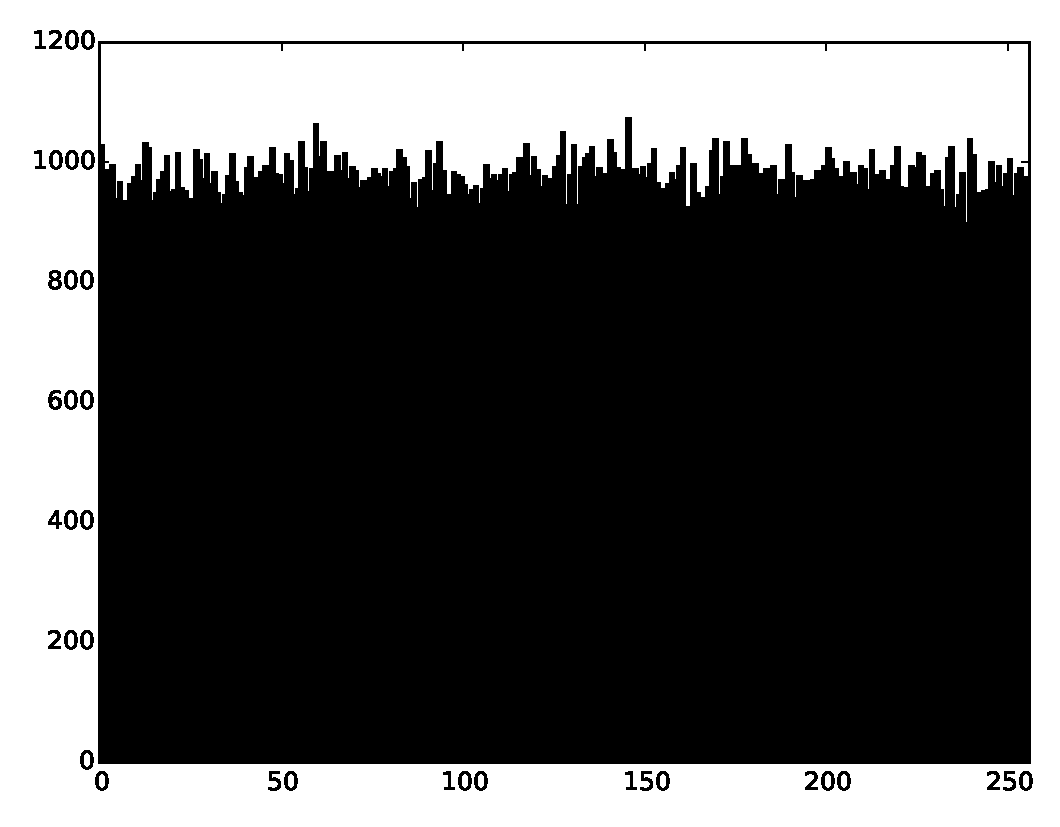
\includegraphics[width=0.520\linewidth]{bilder/uniformnoise_hist.eps}}
  \pnote{Gleichverteilung, annähernd maximale Entropie}
\end{figure}
\end{frame}

\begin{frame}{\insertsubsection}
\begin{figure}[T]
  \centering
  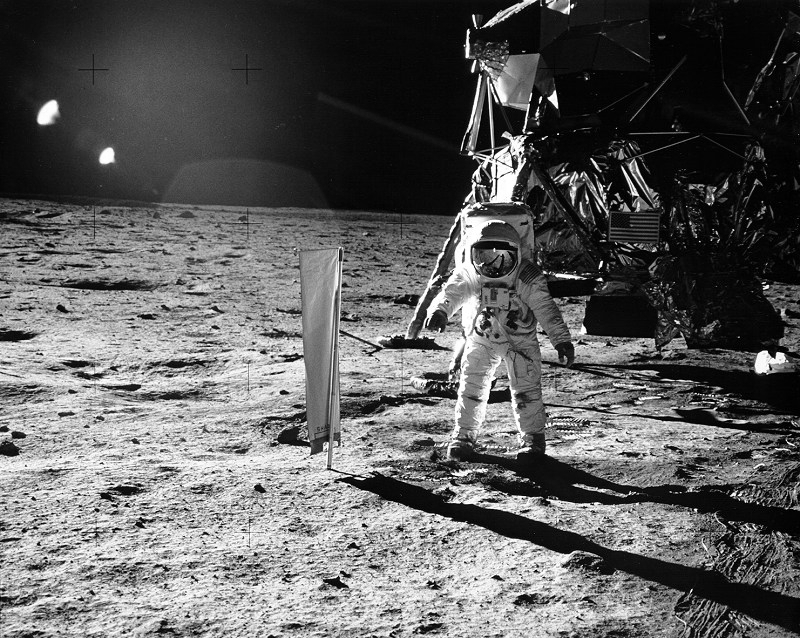
\includegraphics[width=0.470\textwidth]{bilder/moon.jpg}
  \hfill
  \only<2>{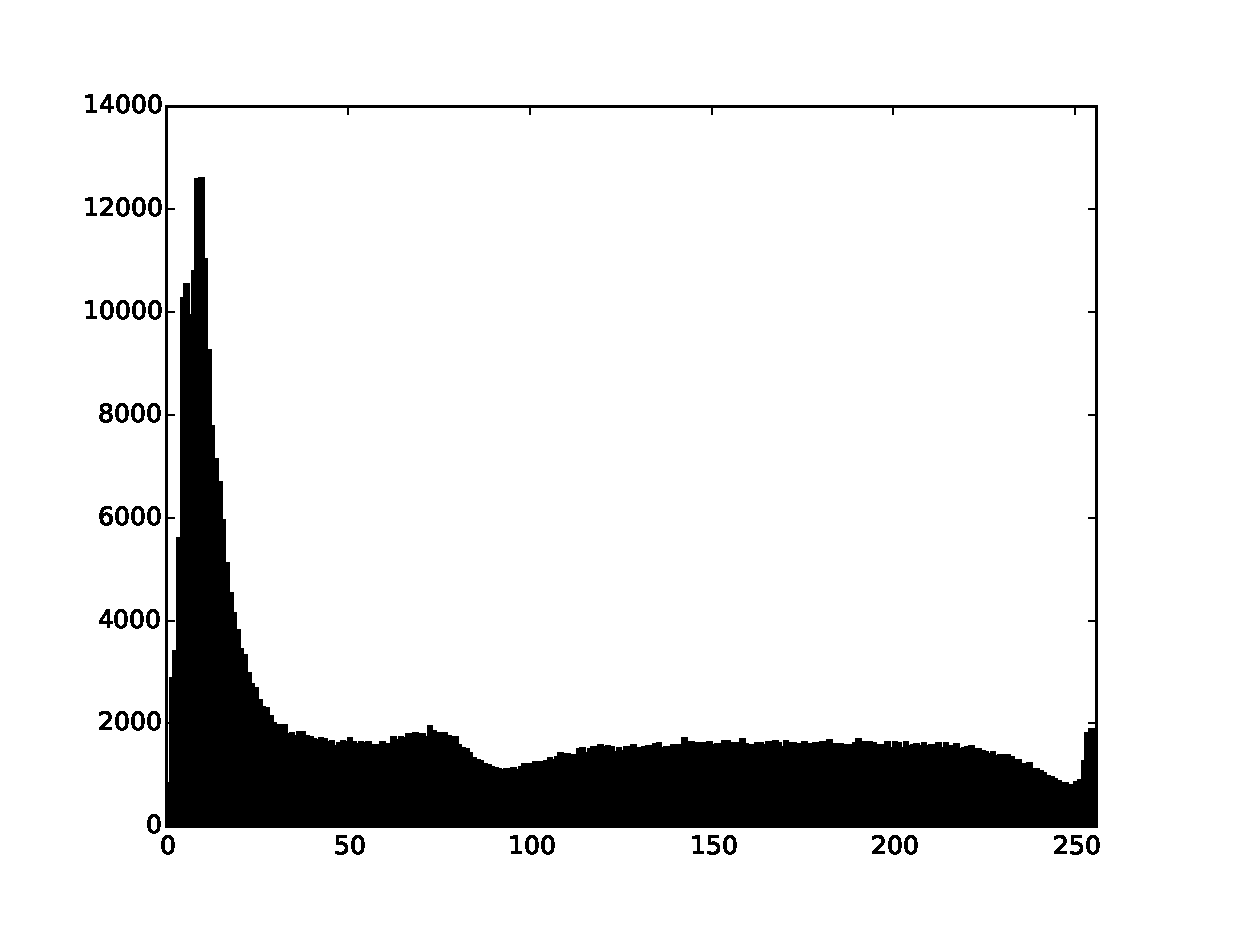
\includegraphics[width=0.520\linewidth]{bilder/moon_hist.eps}}
\end{figure}
\end{frame}

\begin{frame}{\insertsubsection}
  \begin{columns}[T]
    \column{.5\textwidth}
    \begin{tabular}{c|c|l}
      $a_i$ & $H(a_i)$ & $C(a_i)$ \\ \hline
      9 & 12597 & {\tt00100} \\
      8	& 12580 & {\tt00011} \\
      10 & 11018 & {\tt110111} \\
      7	& 10793 & {\tt110110} \\
      \dots & \dots & \dots \\
      247 & 830 & {\tt010101001} \\
      248 & 795 & {\tt010101000} \\
      249 & 784 & {\tt1101010111} \\
      255 & 563 & {\tt1101010110} \\
    \end{tabular}

    \column{.5\textwidth}
    $548680\ \text{Pixel}$ $(800\text{px} \times 638\text{px})$

    \vspace{1em}
    Unkodiert: 8 Bit/Pixel \\
    Kodiert: 7.703 Bit/Pixel

    \vspace{1em}
    Kompressionsrate: 96.3\%

    \vspace{1em}
    548.68kB $\Rightarrow$ 528.34kB
  \end{columns}
\end{frame}

\subsection{Verlustfreie Audiokompression}
\begin{frame}{\insertsubsection}
\begin{witemize}
\item 16-Bit Samples: 65536 verschiedene Eingabesymbole
\item Sehr großer Huffman-Baum
\item Relativ geringe Komprimierung
\item In Realität nicht praktikabel
\end{witemize}
\end{frame}

%%%%%%%%%%%%%%%%%%%%%%%%%%%%%%%%%%%%%%%%%%%%%%%%%%%%%%%%%%%%

\begin{frame}[label=finalSlide]
  \label{LastPage}
  \begin{center}
    \vfill
    {\Large
    \textcolor{i6blue}{Danke für die Aufmerksamkeit!}
    }
     \vfill
     \inserttitle
    \vfill
    {\Large \insertauthor}
    \vfill

    \email{}
  \end{center}
\end{frame}

\end{document}
